\documentclass[../../main.tex]{subfiles}
\begin{document}

{\bf [解]}
\paragraph{(1)}

% TODO: 四面体の図
\begin{figure}[htb]
  \centering
  % 俯角 68°，方位角 115°
  \tdplotsetmaincoords{68}{115}
  \begin{tikzpicture}[tdplot_main_coords, scale=2.5, line join=round, >=stealth, every node/.style={font=\small}]

    % --- 1. 正四面体の頂点座標 ---
    % 底面 BCD (z = 0 平面上の正三角形)
    % 中心を原点とし、外接円半径 1.0
    \coordinate (B) at (0:1.0);           % (1, 0, 0)
    \coordinate (C) at (120:1.0);         % (-0.5, sqrt(3)/2, 0)
    \coordinate (D) at (240:1.0);         % (-0.5, -sqrt(3)/2, 0)

    % 頂点 A (正四面体の一辺長 = sqrt(3) ≈ 1.732, 高さ h = sqrt(2) ≈ 1.414)
    \coordinate (A) at (0, 0, {sqrt(2.0)});

    % --- 2. 各面の薄い透過ハッチング・塗りつぶし ---
    % 底面 BCD (水平面)
    \fill[gray!10, opacity=0.6] (B) -- (C) -- (D) -- cycle;
    % 側面 ABD (手前側)
    \fill[blue!15, opacity=0.6] (A) -- (B) -- (D) -- cycle;
    % 側面 ABC (手前側)
    \fill[teal!12, opacity=0.5] (A) -- (B) -- (C) -- cycle;

    % --- 3. 稜線の描画（奥側の隠れ線を破線に）---
    % 奥側の稜線 CD
    \draw[dashed, gray!60, thick] (C) -- (D);

    % 手前の外枠・稜線
    \draw[very thick, gray!80!black] (B) -- (C);
    \draw[very thick, gray!80!black] (B) -- (D);
    \draw[very thick, gray!80!black] (A) -- (C);
    \draw[very thick, gray!80!black] (A) -- (D);

    % 主経路 AB（導通を考える2端点間の辺を青太線で強調）
    \draw[line width=2.0pt, blue!85!black] (A) -- (B);
    \node[blue!90!black, font=\scriptsize\bfseries, above right] at ($ (A)!0.5!(B) $) {辺 $AB$};

    % --- 4. 端子 A, B への入出力矢印 ---
    % 入力端子 A
    \draw[<-, line width=1.5pt, teal!85!black] (A) -- ($(A) + (0, 0, 0.7)$);
    \node[teal!90!black, font=\footnotesize\bfseries, above] at ($(A) + (0, 0, 0.7)$) {端子 $A$};

    % 出力端子 B
    \draw[->, line width=1.5pt, red!85!black] (B) -- ($(B) + (0.6, 0, 0)$);
    \node[red!90!black, font=\footnotesize\bfseries, right] at ($(B) + (0.6, 0, 0)$) {端子 $B$};

    % --- 5. 頂点プロットとラベル ---
    \fill[teal!85!black] (A) circle (1.2pt) node[left=2pt, font=\normalsize\bfseries, teal!90!black] {$A$};
    \fill[red!85!black]  (B) circle (1.2pt) node[below=2pt, font=\normalsize\bfseries, red!90!black] {$B$};
    \fill[black]         (C) circle (1.0pt) node[above right=1pt] {$C$};
    \fill[black]         (D) circle (1.0pt) node[below left=1pt] {$D$};

    % 各辺の導通確率 p の注記
    \node[gray!70!black, font=\tiny, below=1pt] at ($ (B)!0.5!(D) $) {確率 $p$};
    \node[gray!70!black, font=\tiny, above left=1pt] at ($ (A)!0.5!(D) $) {確率 $p$};

  \end{tikzpicture}
  \caption{正四面体 $ABCD$ }
  \label{fig:tetrahedron_circuit_3d}
\end{figure}

余事象を考える．$A \to B$ に電流が流れないのは，
$AB$ に流れないのもとで，$BD, CB$ に流れるか否かで場合分けする．

\begin{figure}[htb]
  \centering
  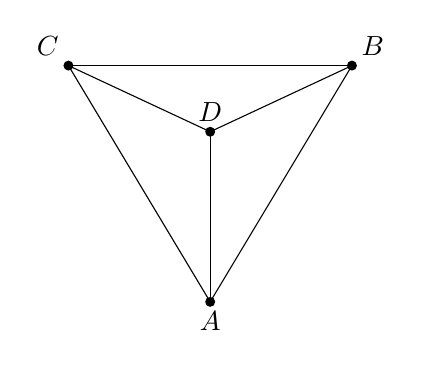
\begin{tikzpicture}[scale=1.2]
    \coordinate (A) at (0,-1);
    \coordinate (B) at (1.5,1.5);
    \coordinate (C) at (-1.5,1.5);
    \coordinate (D) at (0,0.8);
    \draw (A) -- (B);
    \draw (A) -- (C);
    \draw (A) -- (D);
    \draw (B) -- (C);
    \draw (B) -- (D);
    \draw (C) -- (D);
    \fill (A) circle (1.5pt) node[below] {$A$};
    \fill (B) circle (1.5pt) node[above right] {$B$};
    \fill (C) circle (1.5pt) node[above left] {$C$};
    \fill (D) circle (1.5pt) node[above] {$D$};
  \end{tikzpicture}
  \caption{電気回路の配置（点$A,B,C,D$）}
\end{figure}

\begin{table}[htb]
  \centering
  \begin{tabular}{|c|c|c|}
    \hline
    \diagbox{BC}{BD} & 流れる & 流れない \\ \hline
    流れる & $AD, AC$ に流れない．確率$p^2(1-p)^2$ & \shortstack{$AC$ に流れない, \\ $AD, DC$ に同時には流れない \\ 確率$p(1-p)^2(1-p^2)$} \\ \hline
    流れない & \shortstack{$AC$ に流れない, \\ $AD, DC$ に同時には流れない \\ 確率$p(1-p)^2(1-p^2)$} & 任意 確率$(1-p)^2$\\ \hline
  \end{tabular}
  \caption{$BC,BD$の状態による場合分けと，辺$AB$に流れない部分をのぞいた確率．}
\end{table}

上表から，余事象の確率は
\begin{align}
  &(1-p)\left[ p^2(1-p)^2 + 2(1-p)(1-p^2)p(1-p) + (1-p)^2 \right] \\
  &= (1-p)^3 [ p^2 + 2p(1-p^2) + 1 ] = (1-p)^3 (-2p^3 + p^2 + 2p + 1)
\end{align}
だから求める確率は，これを$1$から減じて
\begin{align}
  1 - (1-p)^3(-2p^3 + p^2 + 2p + 1) &= p(1 + 2p - 7p^3 + 7p^4 - 2p^5) \hfill \qed \label{eq:1}
\end{align}
である．

\paragraph{(2)}

% TODO: 四面体ABCD, EFGHがAとEで繋がっている様子
\begin{figure}[htb]
  \centering
  \begin{tikzpicture}[scale=1.5, >=stealth, every node/.style={font=\small}]

    % --- 1. 接続点 (接合頂点 A = E) ---
    \coordinate (A_E) at (0, 0);

    % --- 2. 左側の四面体 ABCD ---
    % 頂点配置: A(=E) が右端、B が左端、C が上、D が手前
    \coordinate (B) at (-3.0, 0.4);
    \coordinate (C) at (-1.8, 1.4);
    \coordinate (D) at (-1.3, -0.8);

    % 左四面体の面（薄い色付け）
    \fill[blue!10, opacity=0.6] (B) -- (C) -- (D) -- cycle;
    \fill[teal!10, opacity=0.6] (A_E) -- (C) -- (D) -- cycle;

    % 左四面体の稜線
    \draw[very thick, gray!75!black]  (B) -- (C);
    \draw[very thick, gray!75!black] (B) -- (D);
    \draw[very thick, gray!75!black] (C) -- (D);
    \draw[very thick, gray!75!black] (A_E) -- (C);
    \draw[very thick, gray!75!black] (A_E) -- (D);
    \draw[line width=1.6pt, blue!85!black] (B) -- (A_E);

    % --- 3. 右側の四面体 EFGH ---
    % 頂点配置: E(=A) が左端、F が右端、G が上、H が手前
    \coordinate (F) at (3.0, 0.4);
    \coordinate (G) at (1.8, 1.4);
    \coordinate (H) at (1.3, -0.8);

    % 右四面体の面（薄い色付け）
    \fill[orange!10, opacity=0.6] (F) -- (G) -- (H) -- cycle;
    \fill[red!10, opacity=0.6] (A_E) -- (G) -- (H) -- cycle;

    % 右四面体の稜線
    \draw[very thick, gray!75!black] (F) -- (G);
    \draw[very thick, gray!75!black] (F) -- (H);
    \draw[very thick, gray!75!black] (G) -- (H);
    \draw[very thick, gray!75!black] (A_E) -- (G);
    \draw[very thick, gray!75!black] (A_E) -- (H);
    \draw[line width=1.6pt, red!85!black] (A_E) -- (F);

    % --- 4. 電流の流れを示す入出力矢印 ---
    % 入力端子 B
    \draw[->, line width=1.6pt, teal!85!black] (-3.8, 0.4) -- (B);
    \node[teal!90!black, font=\footnotesize\bfseries, left] at (-3.8, 0.4) {入力 $B$};

    % 中継点 A=E を通過する矢印
    \draw[->, line width=1.4pt, purple!85!black] (-0.5, 0.2) -- (0.5, 0.2);

    % 出力端子 F
    \draw[->, line width=1.6pt, teal!85!black] (F) -- (3.8, 0.4);
    \node[teal!90!black, font=\footnotesize\bfseries, right] at (3.8, 0.4) {出力 $F$};

    % --- 5. 頂点プロットとラベル ---
    % 接合点 A = E
    \fill[purple!90!black] (A_E) circle (2.0pt);
    \node[below=3pt, font=\normalsize\bfseries, purple!95!black] at (A_E) {$A = E$};

    % 左側の頂点
    \fill[teal!85!black] (B) circle (1.6pt) node[below left=1pt, font=\normalsize\bfseries, teal!90!black] {$B$};
    \fill[black]         (C) circle (1.2pt) node[above=2pt] {$C$};
    \fill[black]         (D) circle (1.2pt) node[below=2pt] {$D$};

    % 右側の頂点
    \fill[teal!85!black] (F) circle (1.6pt) node[below right=1pt, font=\normalsize\bfseries, teal!90!black] {$F$};
    \fill[black]         (G) circle (1.2pt) node[above=2pt] {$G$};
    \fill[black]         (H) circle (1.2pt) node[below=2pt] {$H$};

    % 回路ブロックのラベル
    \node[blue!90!black, font=\footnotesize\bfseries] at (-1.6, -1.3) {四面体回路 $ABCD$};
    \node[red!90!black, font=\footnotesize\bfseries]  at (1.6, -1.3) {四面体回路 $EFGH$};

  \end{tikzpicture}
  \caption{頂点 $A$ と $E$ で接続された 2 つの四面体回路 $ABCD$ と $EFGH$}
  \label{fig:connected_two_tetrahedra}
\end{figure}

$B$から$F$に電流が流れるのは「$AB$間に流れる」かつ「$AF$間に流れる」時である．
これらの事象は独立だから求める確率は\cref{eq:1}より
\begin{align}
  p^2 (1 + 2p - 7p^3 + 7p^4 - 2p^5)^2 \hfill \qed
\end{align}
である．

\newpage

\end{document}
